% !TEX root = ./../../_Thesis.tex

\begin{figure}[htb]
	\centering

	\subfigure{
		
\includegraphics[width=0.17\linewidth]{__Images/04/C_20-200@4x.png}
	}
	~
	\subfigure{
		
\includegraphics[width=0.17\linewidth]{__Images/04/D_20-200@4x.png}
	}
	~
	\subfigure{
		
\includegraphics[width=0.17\linewidth]{__Images/04/H_20-200@4x.png}
	}
	~
	\subfigure{
		
\includegraphics[width=0.17\linewidth]{__Images/04/K_20-200@4x.png}
	}
	~
	\subfigure{
		
\includegraphics[width=0.17\linewidth]{__Images/04/N_20-200@4x.png}
	}
	~
	\subfigure{
		
\includegraphics[width=0.17\linewidth]{__Images/04/O_20-200@4x.png}
	}
	~
	\subfigure{
		
\includegraphics[width=0.17\linewidth]{__Images/04/R_20-200@4x.png}
	}
	~
	\subfigure{
		
\includegraphics[width=0.17\linewidth]{__Images/04/S_20-200@4x.png}
	}
	~
	\subfigure{
		
\includegraphics[width=0.17\linewidth]{__Images/04/V_20-200@4x.png}
	}
	~
	\subfigure{
		
\includegraphics[width=0.17\linewidth]{__Images/04/Z_20-200@4x.png}
	}
	
	\caption{Standard Sloan Letters.}
	\label{fig:sloanletters}
\end{figure}

% section's Name and Label
\section{Target Images and Capture Setup}
\label{sec:CapturingImageInformation}

We have created images of Sloan letters with values ranging from -0.3 to 1.0 in steps of 0.1 in the LogMAR (Logarithm of the Minimum Angle of Resolution) scale \cite{Bailey1976}. Such an interval corresponds to the range from 20/10 to 20/200, respectively, in the Snellen scale. The LogMAR  scale provides a more accurate estimate of visual acuity when compared to other charts (\eg, Snellen), being the recommended one for research settings. 
Our target images were created according to Equation~\ref{eq:lettersize} for testing vision from three feet away. The individual letters were rendered using the vector graphics capabilities of Inkscape and the Sloan PostScript fonts provided by \citet{Pelli1988} 
%. Using the standard Sloan letters, we generated files at 360 dpi, containing black letters on white background 
(Figure~\ref{fig:sloanletters}).
% as well as white letters on black background. 
At the prescribed distance, the ratio between one pixel and one arc minute is 1:1, that is, the letters with a LogMAR value of 0 (or Snellen fraction 20/20) has exactly 5 pixels of height. For the purpose of our simulations, each black (white) letter (also called an {\it optotype}) was placed against a $113 \times 133$-pixel black (white) square.   
Since $1~degree = 60~arc~minutes$, each such square covers a total field of view (FOV) of 1,88� $\times$ 1,88�. The conversion from {\it Snellen decimal acuity} values  
%and vice-versa are 
to LogMAR values is presented in Equation \ref{eq:dec2logmar}. A Snellen decimal acuity value is the decimal representation
of the equivalent Snellen ratio (\eg, Snellen ratios of 20/20 and 20/40 correspond to Snellen decimal acuity values of 1.0 and 0.5, respectively). 
% and \ref{eq:logmar2dec}, respectively.

\begin{equation}
	\centering
	\label{eq:lettersize}
	letter~size_{mm} = \left \{  \tan\left [ deg2rad \left (\frac{5}{60} \right ) \right ] \times (chart~distance_{mm}) \times (10^{-LogMAR})^{-1} \right \}
\end{equation}

\begin{equation}
	\centering
	\label{eq:dec2logmar}
	LogMAR = -\log_{10} (Snellen~decimal~acuity)
\end{equation}

%\begin{equation}
	%\centering
	%\label{eq:logmar2dec}
	%Snellen~Decimal~Acuity = 10^{-LogMAR}
%\end{equation}


%In order to capture images of real scenes, 
We have prepared white- and black-background LogMAR charts containing Sloan letters specifically designed for a viewing distance of three feet (Figure~\ref{fig:etdrs_tables}). The charts were printed at 360 dpi on white paper using a laser printer. We then took pictures of the charts with a DSLR camera. The camera was placed at three feet (91.44 cm) from the chart, with focal length set to 18mm. Since images acquired using this setup respect the 1:1 ratio between pixels and arc minutes, one can crop the squares containing the individual optotypes for further processing.

%\begin{lstlisting}[caption = {For educational purposes}]
%function [ L, P, pt, D ] = calc_Sloan( distance_ft, va_snellen )
%	distance_mm   = ft2mm(distance_ft);
%	syms x;
%	eqn = tan(deg2rad(5/60)) == x / (distance_mm * va_snellen);
%	tmp = solve(eqn, x);
%	x   = double(vpa(tmp));
%	
%	L  = x;					% letter size in mm
%	P  = x/5;				% MAR    size in mm
%	pt = mm2psPT(L);		% font   size (Pages, MacOS editor)
%	D  = distance_mm / 10;  % /10   to return distance in cm
%end
%\end{lstlisting}


\begin{figure}[htb]
	\centering

	\subfigure[]{
		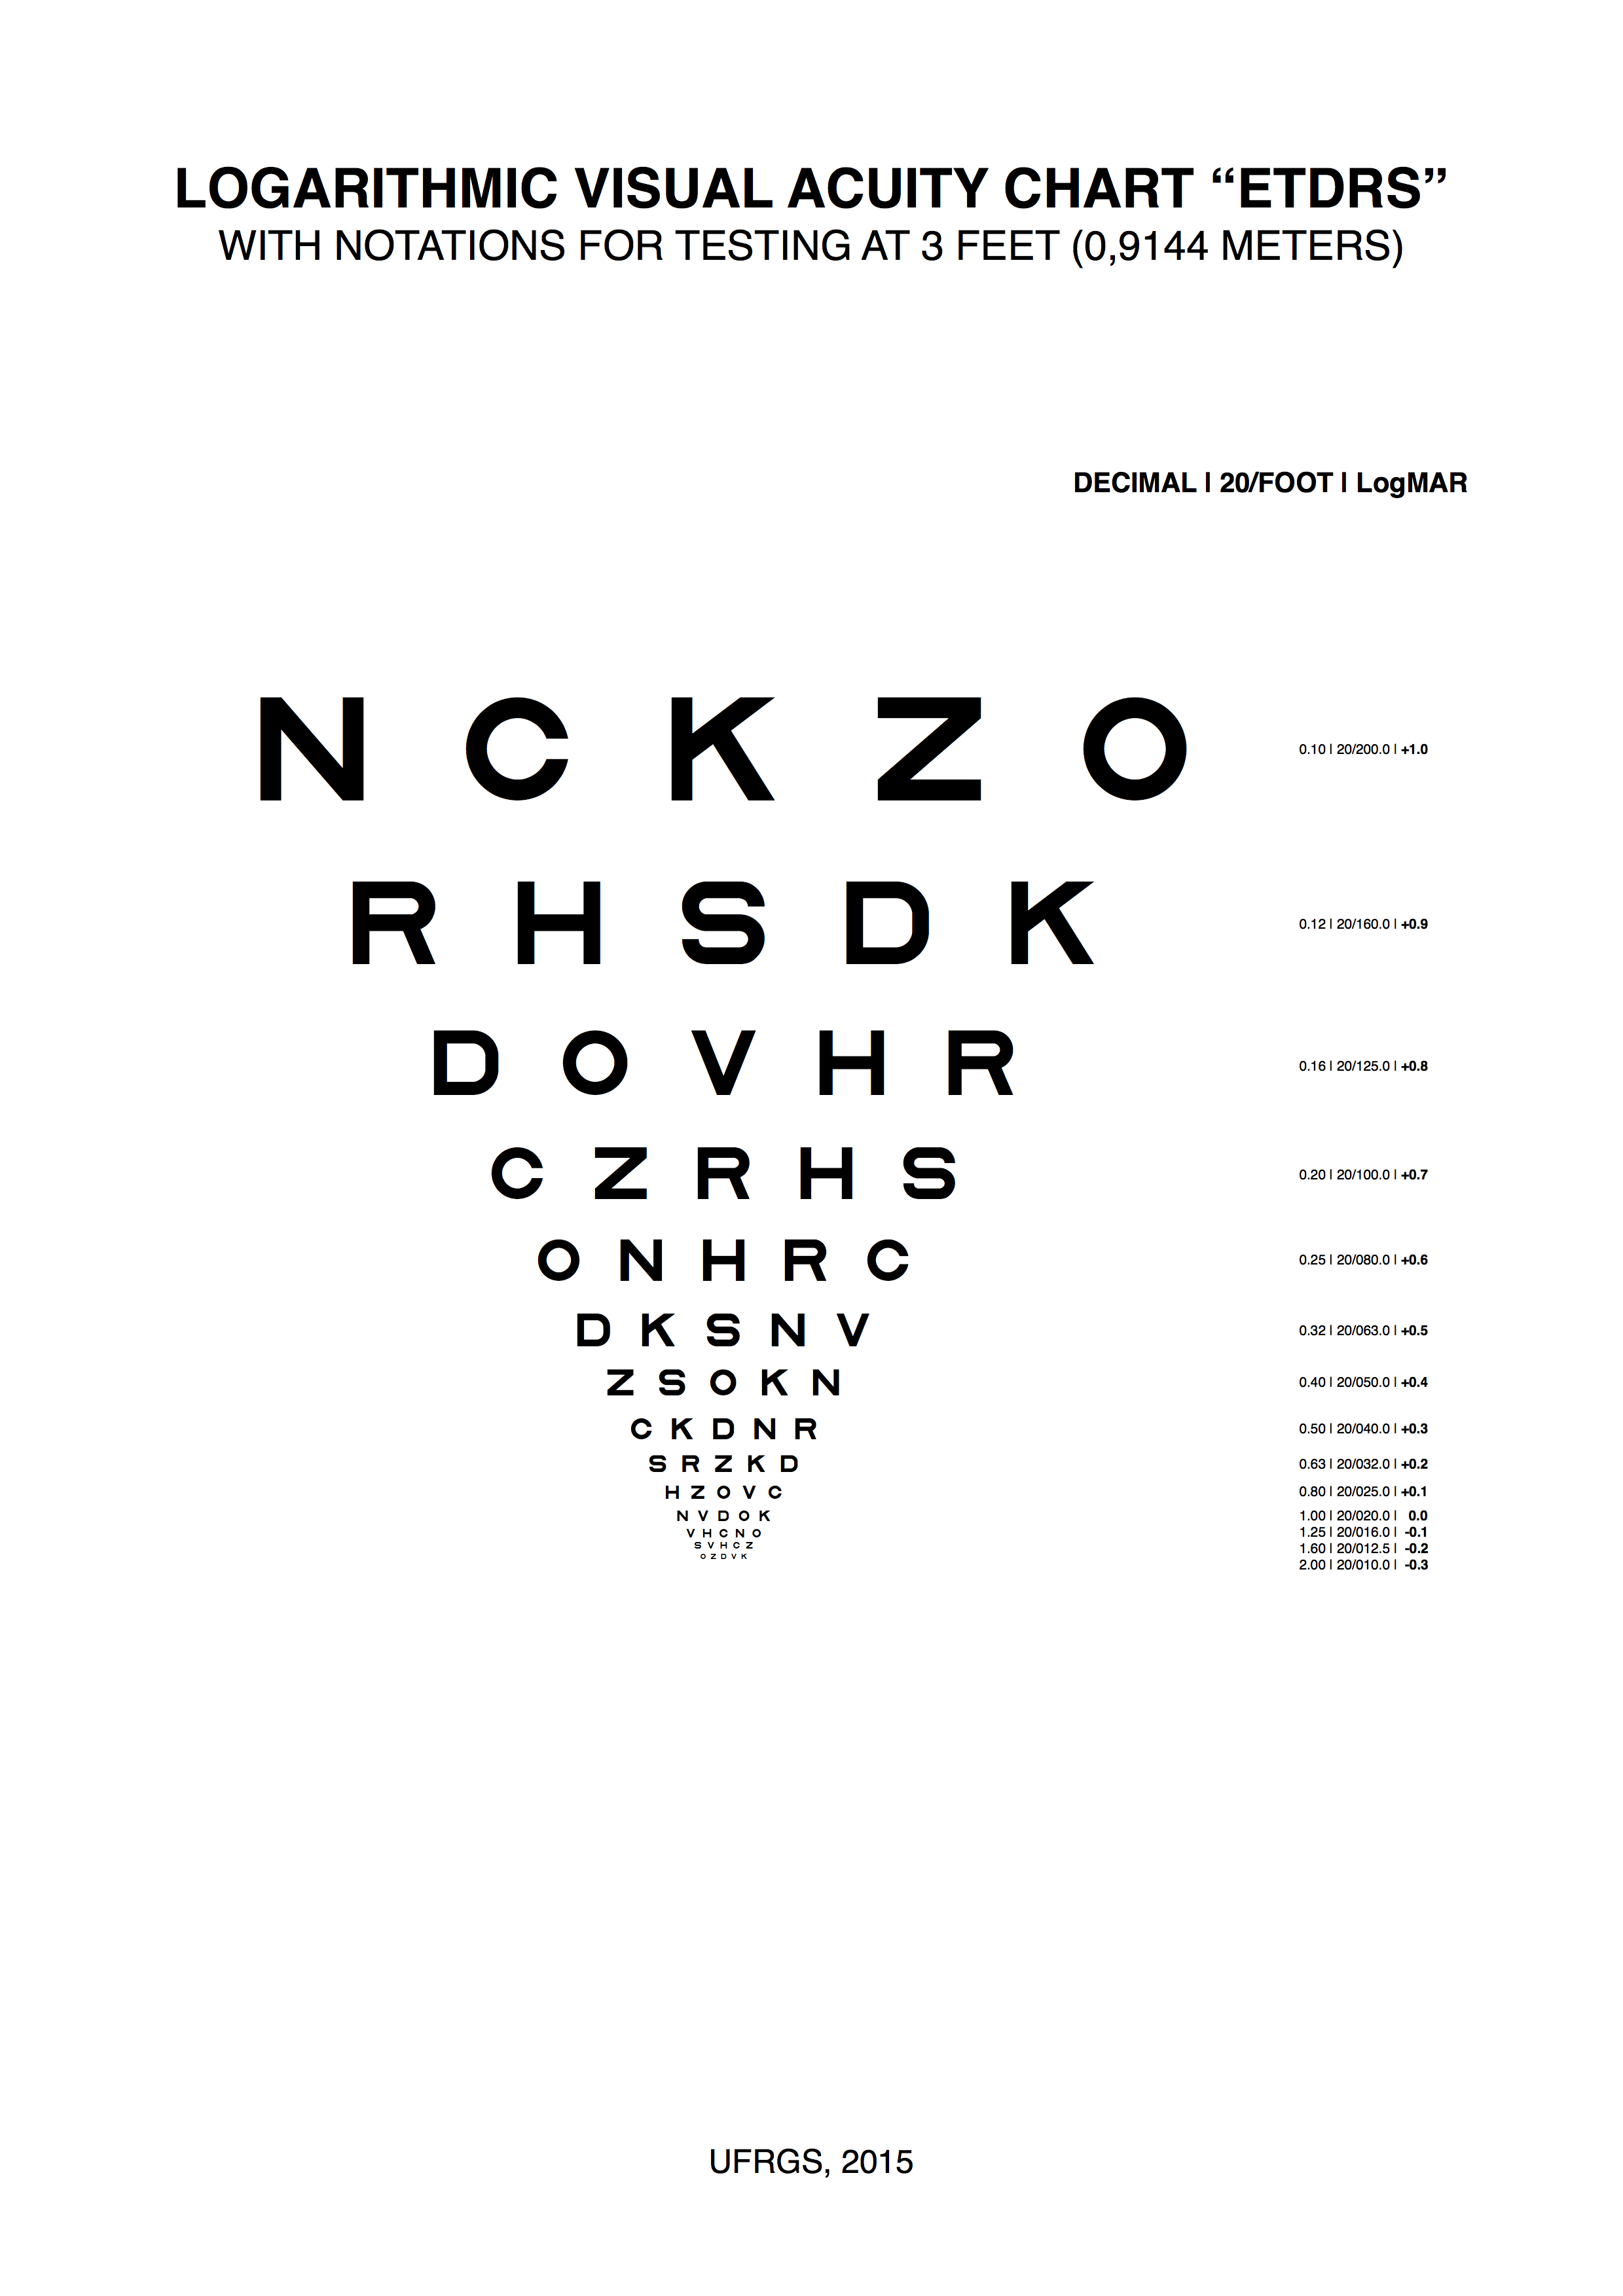
\includegraphics[width=0.45\linewidth]{__Images/04/ETDRS_Chart_W.png}
	}
	~
	\subfigure[]{
		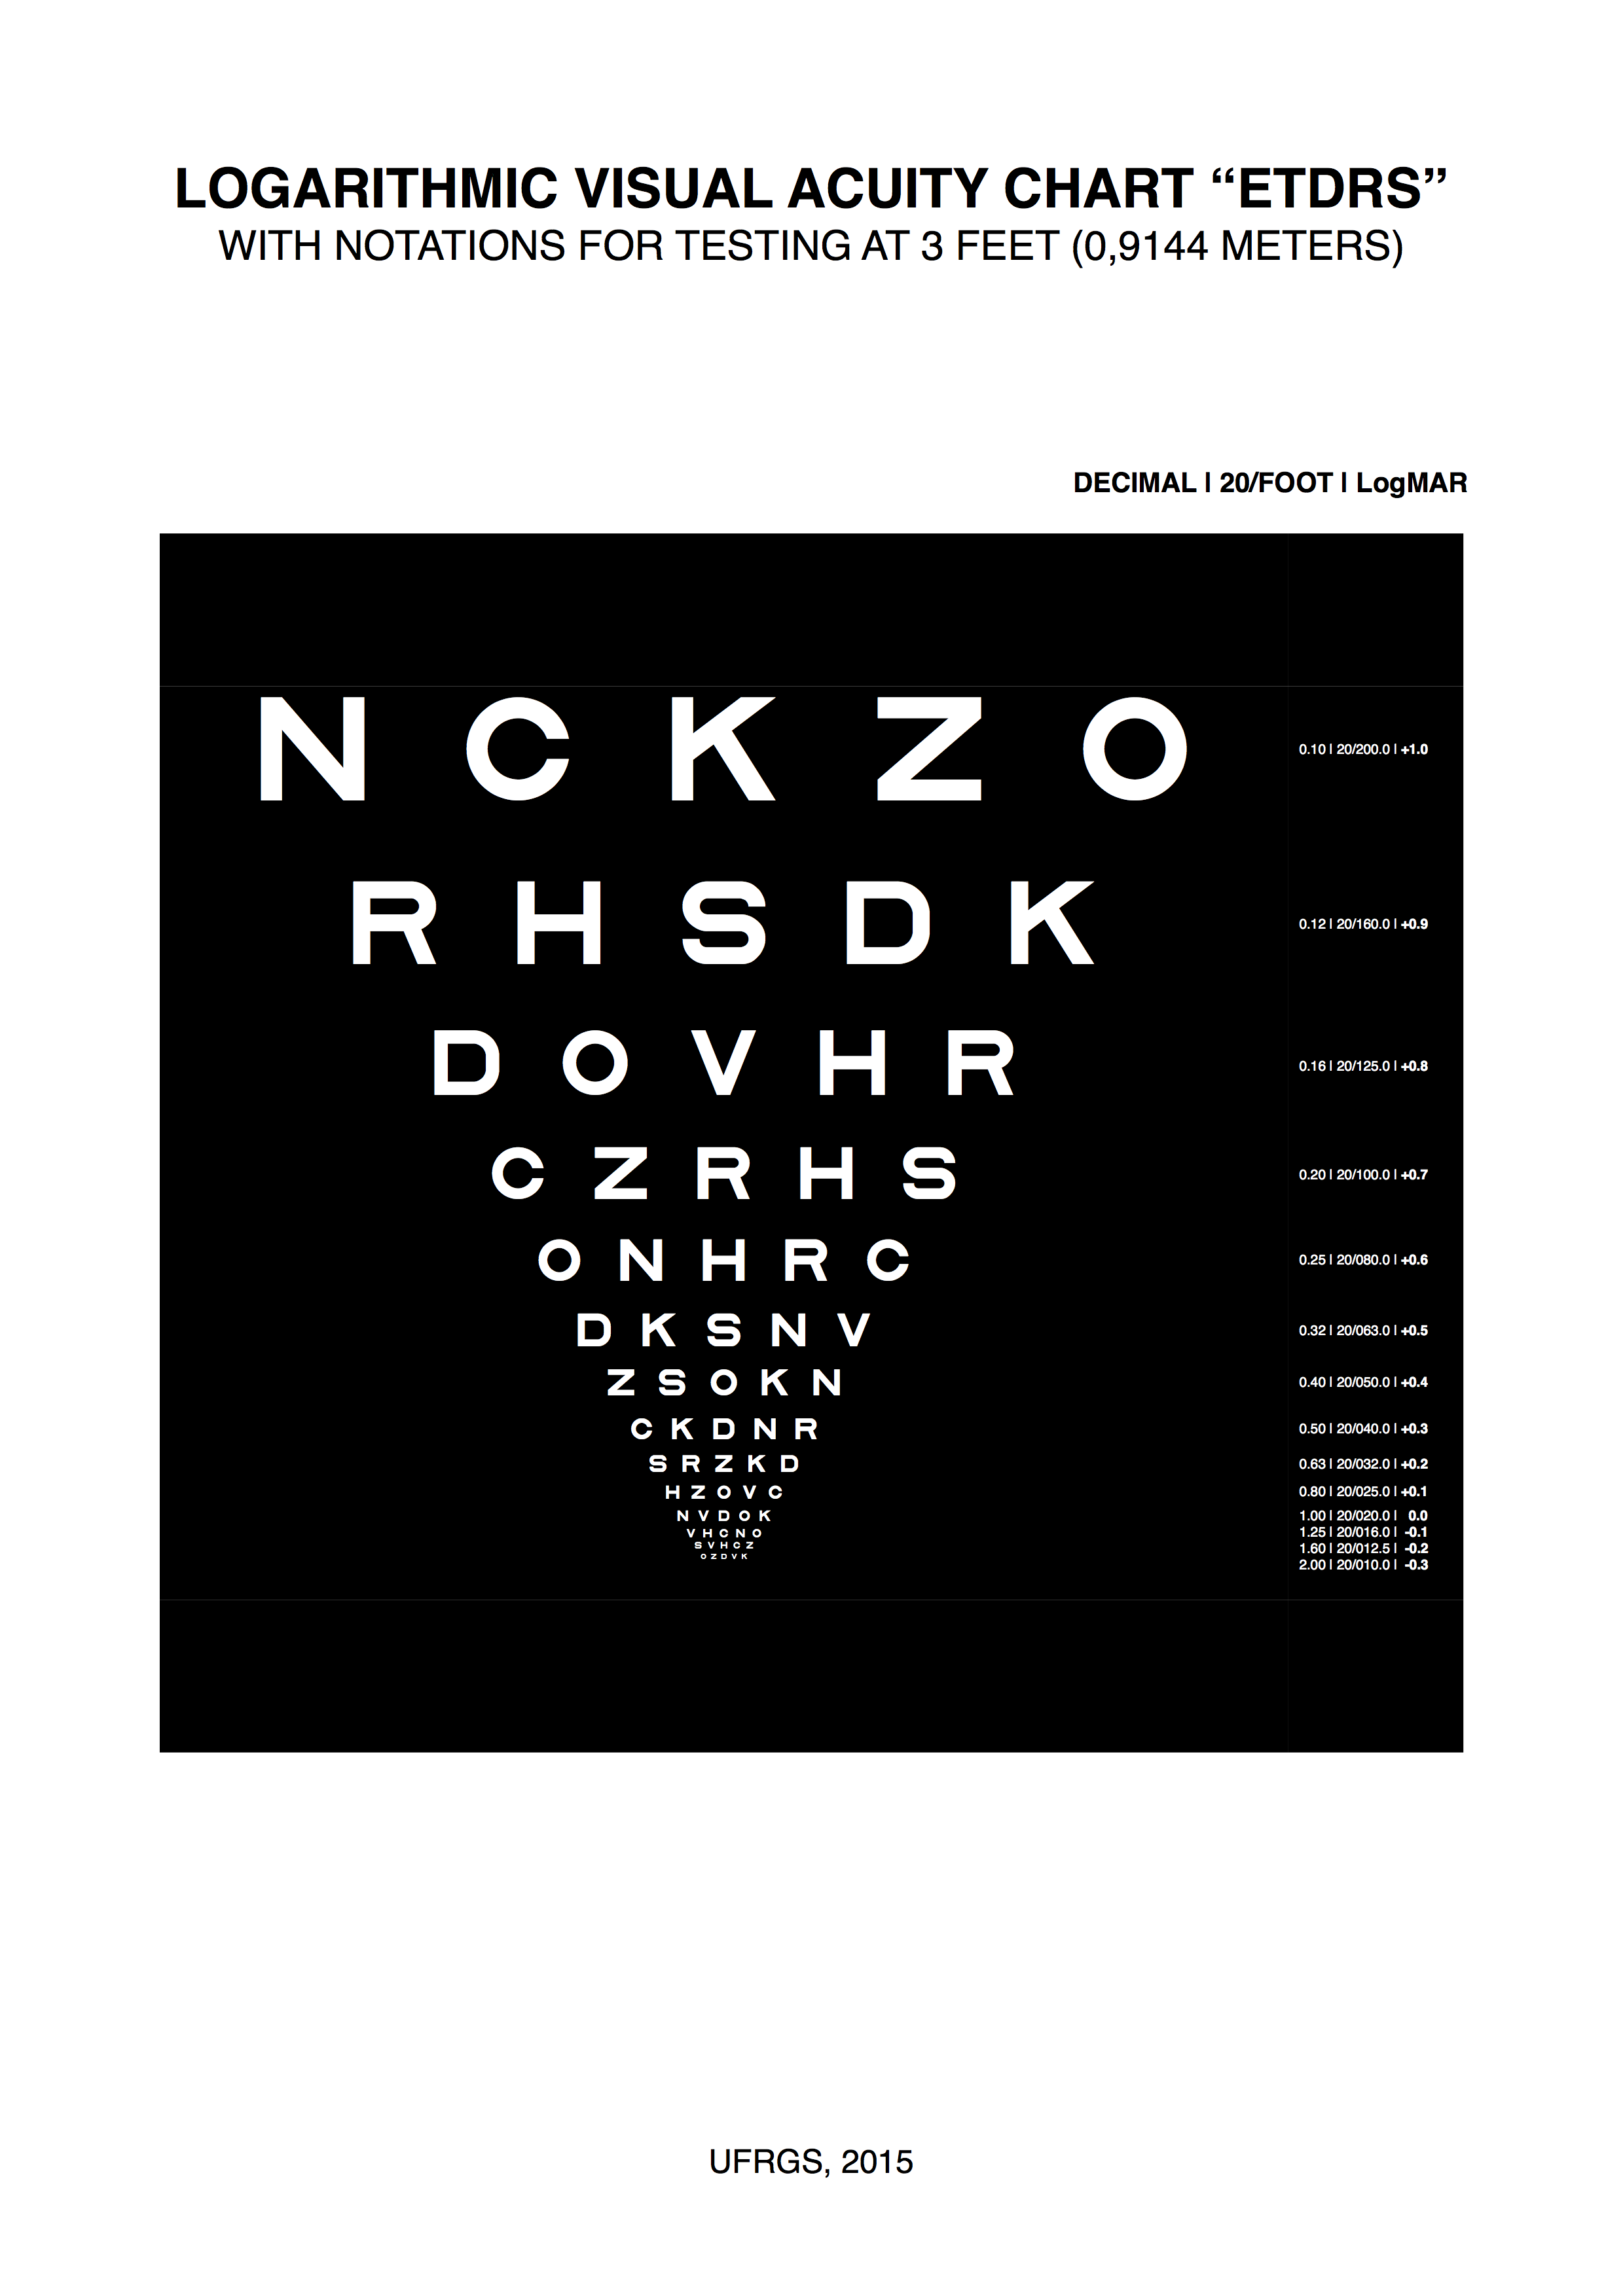
\includegraphics[width=0.45\linewidth]{__Images/04/ETDRS_Chart_B.png}
	}
	
	\caption[LogMAR Charts]{LogMAR charts printed at 360 dpi on white paper using a laser printer. (a) Black letters on white background and (b) white letters on black background. The top row of each table corresponds to Snellen 20/200 (LogMAR +1.0) visual acuity when viewed from three feet. The bottom row corresponds to Snellen 20/10 (LogMAR -0.3) visual acuity when viewed from three feet away.}
	\label{fig:etdrs_tables}
\end{figure}